%% LyX 2.1.3 created this file.  For more info, see http://www.lyx.org/.
%% Do not edit unless you really know what you are doing.
\documentclass[11pt,english]{article}
\renewcommand{\rmdefault}{cmr}
\renewcommand{\sfdefault}{cmss}
\renewcommand{\ttdefault}{cmtt}
\usepackage[T1]{fontenc}
\usepackage[latin9]{inputenc}
\usepackage{geometry}
\geometry{verbose,tmargin=2.5cm,bmargin=2.5cm,lmargin=2.5cm,rmargin=2.5cm}
\setlength{\parskip}{\bigskipamount}
\setlength{\parindent}{0pt}
\usepackage{babel}
\usepackage{amsthm}
\usepackage{amsmath}
\usepackage{amssymb}
\usepackage{setspace}
\setstretch{0.98}
\usepackage[unicode=true,pdfusetitle,
 bookmarks=true,bookmarksnumbered=false,bookmarksopen=false,
 breaklinks=false,pdfborder={0 0 0},backref=false,colorlinks=false]
 {hyperref}

\makeatletter
%%%%%%%%%%%%%%%%%%%%%%%%%%%%%% Textclass specific LaTeX commands.
\theoremstyle{plain}
\newtheorem{thm}{\protect\theoremname}
  \theoremstyle{plain}
  \newtheorem{cor}[thm]{\protect\corollaryname}
  \theoremstyle{plain}
  \newtheorem{lem}[thm]{\protect\lemmaname}
  \theoremstyle{plain}
  \newtheorem{prop}[thm]{\protect\propositionname}
  \theoremstyle{plain}
  \newtheorem{conjecture}[thm]{\protect\conjecturename}
  \theoremstyle{definition}
  \newtheorem{defn}[thm]{\protect\definitionname}
  \theoremstyle{definition}
  \newtheorem{example}[thm]{\protect\examplename}
  \theoremstyle{remark}
  \newtheorem{rem}[thm]{\protect\remarkname}
  \theoremstyle{remark}
  \newtheorem{claim}[thm]{\protect\claimname}

%%%%%%%%%%%%%%%%%%%%%%%%%%%%%% User specified LaTeX commands.
% cleveref allows \ref{thm:asdf} instead of Theorem~\ref{thm:asdf}
\usepackage[nameinlink,capitalise,noabbrev]{cleveref}
\AtBeginDocument{\renewcommand{\ref}[1]{\cref{#1}}}

\usepackage[parfill]{parskip}
\setlength{\parskip}{\bigskipamount}

%have space before theorems
\begingroup
    \makeatletter
    \@for\theoremstyle:=definition,remark,plain\do{%
        \expandafter\g@addto@macro\csname th@\theoremstyle\endcsname{%
            \addtolength\thm@preskip\parskip
            }%
        }
\endgroup

% LyX won't let me include cleveref before theorem declarations so I need to redefine everything as a hack
\theoremstyle{plain}
\newtheorem{mythm}{\protect\theoremname}
\renewenvironment{thm}{\begin{mythm}}{\end{mythm}}
\crefname{mythm}{Theorem}{Theorems}
\theoremstyle{definition}
\newtheorem{mydefn}[mythm]{\protect\definitionname}
\renewenvironment{defn}{\begin{mydefn}}{\end{mydefn}}
\theoremstyle{definition}
\newtheorem{myexample}[mythm]{\protect\examplename}
\renewenvironment{example}{\begin{myexample}}{\end{myexample}}
\theoremstyle{plain}
\newtheorem{myprop}[mythm]{\protect\propositionname}
\renewenvironment{prop}{\begin{myprop}}{\end{myprop}}
\theoremstyle{plain}
\newtheorem{mycor}[mythm]{\protect\corollaryname}
\renewenvironment{cor}{\begin{mycor}}{\end{mycor}}
\theoremstyle{plain}
\newtheorem{mylem}[mythm]{\protect\lemmaname}
\renewenvironment{lem}{\begin{mylem}}{\end{mylem}}
\crefname{mylem}{Lemma}{Lemmas}
\theoremstyle{plain}
\newtheorem{myconjecture}[mythm]{\protect\conjecturename}
\renewenvironment{conjecture}{\begin{myconjecture}}{\end{myconjecture}}
\theoremstyle{remark}
\newtheorem{myrem}[mythm]{\protect\remarkname}
\renewenvironment{rem}{\begin{myrem}}{\end{myrem}}
\theoremstyle{remark}
\newtheorem{myclaim}[mythm]{\protect\claimname}
\renewenvironment{claim}{\begin{myclaim}}{\end{myclaim}}

% equation cref format
\crefformat{equation}{#2(#1)#3}

% \left(\right) should behave the same as ()
\let\originalleft\left
\let\originalright\right
\renewcommand{\left}{\mathopen{}\mathclose\bgroup\originalleft}
\renewcommand{\right}{\aftergroup\egroup\originalright}
\usepackage{pgfplots}
\usetikzlibrary{pgfplots.groupplots}
\usepackage{verbatim}

%make sure tildes in url are vertically centered
\makeatletter
\renewcommand*{\UrlTildeSpecial}{%
  \do\~{%
    \mbox{%
      \fontfamily{ptm}\selectfont
      \textasciitilde
    }%
  }%  
}%    
\let\Url@force@Tilde\UrlTildeSpecial
\makeatother

%graph drawing
\usepackage{tikz}
\usetikzlibrary{external}
\usetikzlibrary{decorations.markings}
\usetikzlibrary{arrows.meta}
\tikzexternalize
\tikzstyle{vertex}=[circle,draw=black,fill=black,inner sep=0,minimum size=0.2cm,text=white,font=\footnotesize]
\tikzset{arc/.style={
        decoration={markings,
            mark= at position 0.5 with {\arrow{Latex[length=2mm,width=2mm]}} ,
        },
        postaction={decorate}
    }
}
\tikzset{every loop/.style={min distance=50,in=50,out=130,looseness=7}}

%caption labels
\usepackage[labelfont=bf,labelsep=period]{caption}

\usepackage{enumitem}

\makeatother

  \providecommand{\claimname}{Claim}
  \providecommand{\conjecturename}{Conjecture}
  \providecommand{\corollaryname}{Corollary}
  \providecommand{\definitionname}{Definition}
  \providecommand{\examplename}{Example}
  \providecommand{\lemmaname}{Lemma}
  \providecommand{\propositionname}{Proposition}
  \providecommand{\remarkname}{Remark}
\providecommand{\theoremname}{Theorem}

\begin{document}

\title{Bounded-degree spanning trees in randomly perturbed graphs}


\author{Michael Krivelevich, Matthew Kwan, Benny Sudakov}

\maketitle
\global\long\def\RR{\mathbb{R}}


\global\long\def\QQ{\mathbb{Q}}


\global\long\def\HH{\mathbb{H}}


\global\long\def\E{\mathbb{E}}


\global\long\def\Var{\operatorname{Var}}


\global\long\def\CC{\mathbb{C}}


\global\long\def\NN{\mathbb{N}}


\global\long\def\ZZ{\mathbb{Z}}


\global\long\def\GG{\mathbb{G}}


\global\long\def\BB{\mathbb{B}}


\global\long\def\DD{\mathbb{D}}


\global\long\def\cL{\mathcal{L}}


\global\long\def\supp{\operatorname{supp}}


\global\long\def\one{\boldsymbol{1}}


\global\long\def\range#1{\left[#1\right]}


\global\long\def\d{\operatorname{d}}


\global\long\def\falling#1#2{\left(#1\right)_{#2}}


\global\long\def\f{\mathbf{f}}


\global\long\def\im{\operatorname{im}}


\global\long\def\sp{\operatorname{span}}


\global\long\def\sign{\operatorname{sign}}


\global\long\def\mod{\operatorname{mod}}


\global\long\def\id{\operatorname{id}}


\global\long\def\disc{\operatorname{disc}}


\global\long\def\lindisc{\operatorname{lindisc}}


\global\long\def\tr{\operatorname{tr}}


\global\long\def\adj{\operatorname{adj}}


\global\long\def\Unif{\operatorname{Unif}}


\global\long\def\Po{\operatorname{Po}}


\global\long\def\Bin{\operatorname{Bin}}


\global\long\def\Ber{\operatorname{Ber}}


\global\long\def\Geom{\operatorname{Geom}}


\global\long\def\Hom{\operatorname{Hom}}


\global\long\def\floor#1{\left\lfloor #1\right\rfloor }


\global\long\def\ceil#1{\left\lceil #1\right\rceil }

\begin{abstract}
abstract
\end{abstract}
\begin{comment}
\begin{thm}
t\end{thm}
\begin{cor}
c\end{cor}
\begin{lem}
l\end{lem}
\begin{prop}
p\end{prop}
\begin{conjecture}
c\end{conjecture}
\begin{defn}
d\end{defn}
\begin{example}
e\end{example}
\begin{rem}
r\end{rem}
\begin{claim}
c
\end{claim}
\end{comment}

\global\long\def\a{\alpha}


\global\long\def\c{c}


\global\long\def\D{\Delta}


\global\long\def\G{G}


\global\long\def\F{F}


\global\long\def\T{T}


\global\long\def\R{R}


\global\long\def\B#1{\BB\left(#1\right)}


We will prove the following theorem.
\begin{thm}
\label{thm:main-theorem}There is $\c=\c\left(\a,\D\right)$ such
that if $\G$ is a graph on the vertex set $\range n$ with minimum
degree at least $\a n$, $\T$ is a tree on $\range n$ with maximum
degree at most $\D$, and $\R\in\GG\left(n,\c/n\right)$, then a.a.s.
$\T\subseteq\G\cup\R$.
\end{thm}
A key ingredient of the proof is the following lemma: with the random
edges in $\R$ alone, we can embed trees that are not too big.
\begin{lem}[{\cite[Theorem~1.1]{AKS07}}]
\label{lem:almost-spanning}There is $\c=\c\left(\varepsilon,\D\right)$
such that $\G\in\GG\left(n,\c/n\right)$ a.a.s. contains every tree
of maximum degree at most $\D$ on $\left(1-\varepsilon\right)n$
vertices.
\end{lem}
We will split the proof of \ref{thm:main-theorem} into two cases
in a similar way to \cite{Kri10}. If our spanning tree $\T$ has
many leaves, then we remove the leaves and embed the resulting non-spanning
tree in $\R$ (using \ref{lem:almost-spanning}). To complete this
into our spanning tree $\T$, it remains to match the the vertices
needing leaves with leftover vertices. This amounts to finding a perfect
matching in a certain bipartite graph. The random edges in $\R$ provide
several almost-perfect matchings on their own; we combine these with
the dense graph $\G$ to satisfy the conditions of Hall's marriage
theorem and guarantee the required perfect matching.

The more difficult case is if $\T$ has few leaves. In this case $\T$
cannot be very ``complicated'' and must be a subdivision of a small
tree. In particular $\T$ must have many long \emph{bare paths}: paths
where each vertex has degree exactly two. By removing some of these
bare paths we can obtain a non-spanning forest. We would like to embed
such a forest into $\R$ using \ref{lem:almost-spanning}, then complete
it into the spanning tree $\T$. This would involve joining up distinguished
pairs of vertices with disjoint paths of certain lengths. In order
to make this task feasible we first use Szemer\'edi's regularity
lemma to divide the vertex set into a bounded number of pieces, each
of which induces a ``super-regular pair'' in $\G$ (that is, a dense
subgraph with edges very well-distributed). When we embed our forest,
some of the paths we need to add will be between pieces, and some
will be within pieces. We carefully choose which bare paths to remove,
and choose how to embed the resulting forest, in such a way that very
few such paths need to be between pieces. We first greedily embed
this small number of paths between pieces. Then the super-regularity
of the pieces allows us to use a tool called the blow-up lemma to
finish joining up the paths, after making some adjustments using the
random edges in $\R$.

Now we proceed to the details of the proof. It is convenient to work
in the model where $\R$ contains each edge with probability $\c n/{n \choose 2}$
independently. We split the random edges into multiple independent
``phases'': say $\R\supseteq\R_{1}\cup\R_{2}\cup\R_{3}\cup\R_{4}$,
where $\R_{i}\in\GG\left(n,\c_{i}/n\right)$ for some large $\c_{i}=\c_{i}\left(\a,\D\right)$
to be determined (these $\c_{i}$ will in turn determine $\c$).

For our first case suppose there are at least $\lambda n$ leaves
in $\T$ (for some $\lambda=\lambda\left(\a\right)>0$ to be determined).
Then consider the tree $\T'$ with some $\lambda n$ leaves removed.
By \ref{lem:almost-spanning} we can embed $\T'$ into $\R_{1}$.
Let $A'$ be the set of vertices of $\T'$ which had a leaf deleted
from them, and let $B$ be the set of $\lambda n$ vertices not part
of $\T'$. We can assume $A'$ and $B$ are uniformly random disjoint
sets of the appropriate size (note $\left|A'\right|\ge\lambda n/\D$
and $\left|B\right|=\lambda n$). For each $b\in B$, the number of
neighbours in $A'$ is hypergeometrically distributed with expected
value at least $\lambda\a n/\D$. Let $\beta=\lambda\a/\left(2\D\right)$;
by a concentration inequality (for example, see \cite[Theorem 2.10]{JLR00})
and the union bound, a.a.s. each $a'\in A'$ has at least $\beta n$
neighbours in $B$. Similarly each $b\in B$ a.a.s. has at least $\beta n$
neighbours in $A'$. From now on we treat $A'$ and $B$ as fixed
sets satisfying these properties.

For any graph $H$ on $\range n$, we define a bipartite graph $\B H$
by throwing away all edges not between $B$ and $A'$, then making
multiple copies of the vertices in $A'$. Specifically, let $A$ be
a set consisting of $\ell$ copies of each vertex $a'\in A'$ which
needs $\ell$ extra leaves (so $\left|A\right|=\lambda n$). Let $\B H$
be the bipartite graph on the vertex set $A\cup B$ which has an edge
between $a\in A$ (a copy of $a'\in A'$) and $b\in B$ if there is
an edge between $a'$ and $b$ in $\B H$. If we can find a perfect
matching in $\B{\G}\cup\B{\R_{2}}\subseteq\B{\G\cup\R}$, this gives
us a way to extend our embedding of $\T'$ to an embedding of $\T$,
as desired.

Let $\BB_{A,B}\left(p\right)$ be the random binomial graph where
each of the $\left|A\right|\left|B\right|$ possible edges between
$A$ and $B$ are present with probability $p$. For any $\c_{\BB}$,
we can choose large $\c_{2}$ such that $1-\c_{2}/n\le\left(1-\c_{\BB}/n\right)^{\Delta}$
for large $n$. This means $\B{\R_{2}}$ stochastically dominates
$\BB_{A,B}\left(\c_{\BB}/n\right)$, so the following lemma provides
the desired perfect matching.
\begin{lem}
\label{lem:bipartite-perfect-matching}Let $A$ and $B$ be $n$-vertex
sets. There is $\c_{\BB}=\c_{\BB}\left(\a\right)$ such that if $\G$
is a bipartite graph with bipartition $A\cup B$ and minimum degree
at least $\a n$, and if $\R\in\BB_{A,B}\left(\c_{\BB}/n\right)$,
then a.a.s. $\G\cup\R$ has a perfect matching.
\end{lem}
In order to prove \ref{lem:bipartite-perfect-matching} we need another
lemma.
\begin{lem}
\label{lem:bipartite-matching}Let $\varepsilon>0$, and let $A$
and $B$ be $n$-vertex sets. There is $\c=\c\left(\varepsilon\right)$
such that $\R\in\BB_{A,B}\left(\c/n\right)$ has a matching of size
$\left(1-\varepsilon\right)n$.\end{lem}
\begin{proof}
For any subsets $A'$ and $B'$ of size $\varepsilon n$, the probability
there is no edge between $A'$ and $B'$ is $\left(1-p\right)^{\left(\varepsilon n\right)^{2}}\le e^{-\c\varepsilon^{2}n}$.
There are at most $2^{2n}$ choices of such $A',B'$, so for large
$\c$, by the union bound there is a.a.s. an edge between any such
pair of sets. It follows that a maximum-size matching a.a.s. has at
least $\left(1-\varepsilon\right)n$ edges.
\end{proof}

\begin{proof}[Proof of \ref{lem:bipartite-perfect-matching}]
We apply Hall's marriage theorem. If $W\subseteq A$ with $\left|W\right|\le\a n$
then $\left|N_{\G}\left(W\right)\right|\ge\a n\ge\left|W\right|$
by the minimum degree condition on $\G$. Similarly, every vertex
outside $N_{\G}\left(W\right)$ has at least $\a n$ neighbours outside
$W$, so if $\left|W\right|\ge\left(1-\a\right)n$ then $\left|N_{\G}\left(W\right)\right|=n\ge\left|W\right|$.
So, consider any $W$ with $\a n\le\left|W\right|\le\left(1-\a\right)n$.
Split $\R$ into phases $\R\supseteq\R_{1}\cup\dots\cup\R_{r}$, with
$\R_{i}\in\BB_{A,B}\left(\c'/n\right)$, for some $\c'=\c'\left(\a\right)$
and $r=r\left(\a\right)$ to be determined. By \ref{lem:bipartite-matching},
if $\c'$ is large we can find a $\left(1-\a/2\right)n$-edge matching
$M_{i}$ in each $\R_{i}$. Condition on the vertices $W_{i}:=W\cap M_{i}$
matched by each $M_{i}$. The distribution of $\R_{1}$ is invariant
under permutations of $B$, so we can assume each $N_{M_{i}}\left(W\right)$
is an independently and uniformly random $\left|W_{i}\right|$-element
subset of $B$. We will use this kind of argument implicitly throughout
this paper, to assume that objects embedded in random graphs are themselves
random.

\textbf{Is this OK, or do you think I should explain these symmetry
arguments more?}

For each $b\in B$, let $X_{b,i}$ be the indicator random variable
for the event that $b\notin N_{M_{i}}\left(W\right)$. The random
variables $X_{b,i}$ are said to be \emph{negatively associated} (see
\cite{JDP83}, in particular property $P_{7}$ and Application 3.1(c)).
Hence, the random variables $X_{b}=\min_{i}X_{b,i}$ (which are indicators
for the events $b\notin N_{G}\left(W\right)$) are also negatively
associated. This means in particular that we can apply Chernoff bounds
even though the $X_{b}$ are not independent. We have 
\[
\E\sum_{b\in B}X_{b}=n\prod_{i=1}^{r}\left(\left(n-\left|W_{i}\right|\right)/n\right)\le\left(1-\a/2\right)^{r}n,
\]
so by the Chernoff bound, 
\[
\Pr\left(\left|N\left(W\right)\right|<\left|W\right|\right)=\Pr\left(\sum_{b\in B}X_{b}>n-\left|W\right|\right)\le\Pr\left(\sum_{b\in B}X_{b}>\a n\right)=\exp\left(-\Omega\left(\left(1-\a/2\right)^{-r}\a^{2}\right)\right).
\]
since there are at most $2^{n}$ choices for $W$, for large $r$
the union bound gives $\left|N_{\R}\left(W\right)\right|\ge\left|W\right|$
for all required $W$.
\end{proof}
Now we address the second case where there are fewer than $\lambda n$
leaves in $\T$. As outlined, we first need to divide the vertex set
into groups such that the edges of $\G$ are well distributed within
those groups.

\global\long\def\h{h}

\begin{defn}
For a disjoint pair of vertex sets $\left(X,Y\right)$ in a graph,
let its \emph{density} $d\left(X,Y\right)$ be the number of edges
between $X$ and $Y$, divided by $\left|X\right|\left|Y\right|$.
A pair of vertex sets $\left(V_{1},V_{2}\right)$ is said to be \emph{$\varepsilon$-regular}
if for any $U_{1},U_{2}$ with $U_{\h}\subseteq V_{\h}$ and $\left|U_{\h}\right|\ge\varepsilon\left|V_{\h}\right|$,
we have $\left|d\left(U_{1},U_{2}\right)-d\left(V_{1},V_{2}\right)\right|\le\varepsilon$.
If alternatively $d\left(U_{1},U_{2}\right)\ge\delta$ for all such
pairs $U_{1},U_{2}$ then we say $\left(V_{1},V_{2}\right)$ is \emph{$\left(\varepsilon,\delta\right)$-semi-super-regular}.
Let $\bar{\h}=2-\h$; if $\left(V_{1},V_{2}\right)$ is $\left(\varepsilon,\delta\right)$-semi-super-regular
and moreover each $v\in V_{\h}$ has at least $\delta\left|V_{\bar{\h}}\right|$
neighbours in $V_{\bar{\h}}$, then we say $\left(V_{1},V_{2}\right)$
is \emph{$\left(\varepsilon,\delta\right)$-super-regular}.
\end{defn}
\textbf{Is there already some word to describe what I'm calling ``semi-super-regularity''?
It is basically a one-sided version of regularity.}

\global\long\def\h{h}

\begin{lem}
\label{lem:partition-into-blobs}For $\a,\varepsilon>0$ with $\varepsilon$
sufficiently small relative to $\a$, there are $\delta=\delta\left(\a\right)>0$,
$M=M\left(\a,\varepsilon\right)$, $a=a\left(\a,\varepsilon\right)>0$
and $b=b\left(\a,\varepsilon\right)>0$ such that the following holds.
Let $\G$ be a graph on $\range n$ with minimum degree at least $\a n$.
We can choose $q\le M$ and partition $\range n$ into sets $V_{i}^{\h}$
($1\le i\le q$, $\h=1,2$) such that each $an\le\left|V_{i}^{\h}\right|\le bn$
and each pair $\left(V_{i}^{1},V_{i}^{2}\right)$ is $\left(\varepsilon,\delta\right)$-super-regular.
\end{lem}
To prove \ref{lem:partition-into-blobs}, we apply Szemer\'edi's
regularity lemma to obtain a reduced \emph{cluster graph}, then decompose
this cluster graph into small stars with the following auxiliary lemma,
each of which will roughly correspond to a pair $\left(V_{i}^{1},V_{i}^{2}\right)$.
We will then redistribute some of the vertices to ensure super-regularity.
\begin{lem}
\label{lem:star-cover}Let $G$ be an $n$-vertex graph with minimum
degree at least $\a n$. Then there is a spanning subgraph $Q$ which
is a disjoint union of vertex-disjoint stars, each with at least two
vertices and at most $1/\a$ leaves.\end{lem}
\begin{proof}
Let $Q$ be a maximal-size union of such stars. Suppose there is a
vertex $v$ uncovered by $Q$. If $v$ has a neighbour which is a
centre of one of the stars in $Q$, and that star has fewer than $1/\a$
leaves, then we could add $v$ to that star, contradicting maximality.
Otherwise, if $v$ has a neighbour $w$ which is a leaf of one of
the stars in $Q$, then we could remove that leaf from its star and
create a new 2-vertex star with edge $vw$, again contradicting maximality.
The remaining case is where each of the (at least $\a n$) neighbours
of $v$ is a centre of a star with $1/\a$ leaves. But these stars
would comprise more than $n$ vertices, which is again a contradiction.
We conclude that $Q$ covers $G$, as desired.
\end{proof}

\begin{proof}[Proof of \ref{lem:partition-into-blobs}]
We apply the ``degree form'' of Szemer\'edi's regularity lemma
(\cite[Theorem~1.10]{KS96}) with density threshold $\a'=\a/3$ and
some regularity parameter $\varepsilon'$, which we will repeatedly
assume is very small relative to $\a'$. There is large $M=M\left(\a\right)$,
a partition of $\range n$ into clusters $V_{0},\dots,V_{k}$ ($k\le M$)
and a subgraph $\G'\subseteq\G$ satisfying the following conditions.
The ``exceptional cluster'' $V_{0}$ has size at most $\varepsilon'n$,
and the other clusters have equal size $sn$ (so $1-\varepsilon'\le ks\le1$).
The minimum degree of $\G'$ is at least $\left(\a'+\varepsilon'\right)n$.
There are no edges of $\G'$ within clusters, and each pair of non-exceptional
clusters is $\varepsilon'$-regular in $\G'$ with density at least
$\a'$.

Define the cluster graph $C$ as the bipartite graph whose vertices
are the non-exceptional clusters $V_{i}$, and whose edges are the
pairs of clusters between which there is nonzero density in $G'$.
The fact that $G$ is dense implies that $C$ is dense as well, as
follows. In $\G'$ each $V_{i}$ has at least $\left(\left(\a'+\varepsilon'\right)n\right)\left(sn\right)$
edges to other clusters. There are at most $\left(\varepsilon'n\right)\left(sn\right)$
edges to the exceptional cluster $V_{0}$ and at most $\left(sn\right)^{2}$
edges to each other cluster. So, $d_{C}\left(V_{i}\right)\ge\left(\left(\a'+\varepsilon\right)n-\varepsilon'n\right)sn/\left(sn\right)^{2}\ge\a'k$.
That is, $C$ has minimum degree at least $\a'k$.

Now, let $Q$ be a star cover of $C$ by stars $T_{1},\dots,T_{q}$
of size at most $1/\a'$, as guaranteed by \ref{lem:star-cover}.
Let $W_{i}^{1}$ be the centre cluster of $T_{i}$, and let $W_{i}^{2}$
be the union of the leaf clusters of $T_{i}$ (for two-vertex stars,
arbitrarily choose one vertex as the ``leaf'' and one as the ``centre'').
Consider any $U^{\h}\subseteq W_{i}^{\h}$ with $\left|U^{\h}\right|\ge\varepsilon'W_{i}^{\h}$,
and let $\ell$ be the number of leaves in $T_{i}$. Let $V_{p}$
be the leaf of $T_{i}$ with the most vertices in $U^{2}$, so that
$\left|U^{2}\cap V_{p}\right|\ge\left|U^{2}\right|/\ell\ge\varepsilon'sn$.
By $\varepsilon'$-regularity there are at least $\left(\a'-\varepsilon'\right)\left|U^{1}\right|\left(\left|U^{2}\right|/\ell\right)\ge\left(\left(\a'\right)^{2}/2\right)\left|U^{1}\right|\left|U^{2}\right|$
edges between $U^{2}\cap V_{p}$ and $U^{1}$. That is, $d\left(U^{1},U^{2}\right)\ge\left(\a'\right)^{2}/2$,
so with $\delta'=\left(\a'\right)^{2}/2$ each pair $\left(W_{i}^{1},W_{i}^{2}\right)$
is $\left(\varepsilon',\delta'\right)$-semi-super-regular.

There are still some vertices left over from exceptional clusters,
and we cannot guarantee that the $\left(W_{i}^{1},W_{i}^{2}\right)$
are super-regular (there may be vertices without enough neighbours
in their ``partner'' cluster). We now make some adjustments to fix
these problems.

If $D_{i}^{\h}$ is the set of vertices of $W_{i}^{\h}$ with degree
less than $\delta'\left|W_{i}^{\bar{\h}}\right|$, then there are
fewer than $\delta'\left|D_{i}^{\h}\right|\left|W_{i}^{\bar{\h}}\right|$
edges between $D_{i}^{\h}$ and $W_{i}^{\bar{\h}}$. So, we must have
$\left|D_{i}^{\h}\right|<\varepsilon'\left|W_{i}^{\h}\right|$, by
semi-super-regularity. Let $S_{i}^{\h}=W_{i}^{\h}\backslash D_{i}^{\h}$.
Note that each $v\in S_{i}^{\h}$ has at least $\left(1-\varepsilon\right)\delta'\left|S_{i}^{\h}\right|\ge\delta'\left|S_{i}^{\h}\right|/2$
neighbours in its partner cluster $S_{i}^{\bar{\h}}$. Now, let $V_{i}^{\h}$
correspond to a ``maximal extension'' of the clusters $S_{i}^{\h}$,
as follows. Each $V_{i}^{\h}\supseteq S_{i}^{\h}$, each $V_{i}^{\h}$
is disjoint, each $v\in V_{i}^{\h}$ has at least $\delta'\left|S_{i}^{\bar{\h}}\right|/2$
neighbours in its partner cluster $V_{i}^{2-\h}$, each $\left|V_{i}^{\h}\backslash S_{i}^{\h}\right|\le\left(4\varepsilon'/\a'\right)\left|V_{i}^{\h}\right|$,
and none of the $V_{i}^{\h}$ can be enlarged retaining these properties.

Let $P=V_{0}\cup\bigcup_{i=1}^{q}\left(D_{i}^{1}\cup D_{i}^{2}\right)$
be the set of at most $2\varepsilon'n$ vertices not in any $S_{i}^{\h}$.
If $\left|V_{i}^{\h}\backslash S_{i}^{\h}\right|=\left(4\varepsilon'/\a'\right)\left|V_{i}^{\h}\right|$
then we say $V_{i}^{\h}$ is ``full''. There can be at most $2\varepsilon'n/\left(4\varepsilon'/\a'\right)=\a'n/2$
vertices in full clusters. Now suppose there is some $v$ not in any
$V_{i}^{\h}$. That $v$ has $\a'n/2$ neighbours in non-full clusters,
so some non-full cluster $V_{i}^{\h}$ has $\a'\left|V_{i}^{\h}\right|/2\ge\delta'\left|S_{i}^{\h}\right|/2$
of these neighbours. But this is a contradiction, because we could
add $v$ to $V_{i}^{\bar{\h}}$ and it would still satisfy all the
required properties, contradicting maximality.

We conclude that the $V_{i}^{\h}$ partition the vertex set. If $a=s\left(1-\varepsilon'\right)$
and $b=s/\left(\a'\left(1-4\varepsilon'/\a'\right)\right)$, then
each $an\le\left|V_{i}^{\h}\right|\le bn$. For each $i$, if $U^{\h}\subseteq V_{i}^{\h}$
with $\left|U^{\h}\right|\ge\left(4/\a'+1\right)\varepsilon'\left|V_{i}^{\h}\right|$,
then $\left|U^{\h}\cap W_{i}^{\h}\right|\ge\varepsilon'\left|W_{i}^{\h}\right|$
so
\[
d\left(U^{1},U^{2}\right)\ge d\left(U^{1}\cap W_{i}^{1},U^{2}\cap W_{i}^{2}\right)/\left(4/\a'+1\right)^{2}\ge\delta'/\left(4/\a'+1\right)^{2}.
\]
That is, each pair $\left(V_{i}^{1},V_{i}^{2}\right)$ is $\left(\left(4/\a'+1\right)\varepsilon',\delta\right)$-semi-super-regular,
for $\delta=\delta'/\left(4/\a'+1\right)^{2}$. Finally, each $v\in V_{i}^{\h}$
has at least $\delta'\left|S_{i}^{\bar{\h}}\right|/2\ge\delta'\left|V_{i}^{\bar{\h}}\right|/\left(2\left(4\varepsilon'/\a'+1\right)\right)\ge\delta\left|V_{i}^{\h}\right|$
neighbours in its partner cluster $V_{i}^{\h}$, so in fact each pair
$\left(V_{i}^{1},V_{i}^{2}\right)$ is $\left(\left(4/\a'+1\right)\varepsilon',\delta\right)$-super-regular.
With $\varepsilon'$ small enough so that $\left(4/\a'+1\right)\varepsilon'\le\varepsilon$,
we are done.
\end{proof}
We apply \ref{lem:partition-into-blobs} to our graph $\G$, with
$\varepsilon=\varepsilon\left(\delta\right)$ to be determined. Proceeding
with the proof outline, we need the fact that $\T$ is almost entirely
composed of bare paths, as is guaranteed by the following lemma.
\begin{lem}[{\cite[Lemma~2.1]{Kri10}}]
\label{lem:bare-paths-if-no-leaves}Let $\T$ be a tree on $n$ vertices
with at most $\ell$ leaves. Then $\T$ contains a collection of at
least $\left(n-\left(2\ell-2\right)\left(k+1\right)\right)/\left(k+1\right)$
vertex-disjoint bare paths of length $k$ each.
\end{lem}
\global\long\def\r#1{r\left(#1\right)}


In our case $\ell=\lambda n$. For any $\phi=\phi\left(\a\right)>0$
(which we will determine later), if we choose $k=k\left(\phi\right)$
large enough and $\lambda=\lambda\left(k\right)$ small enough, then
$\T$ contains a collection of $\left(1-\phi\right)n/\left(k-1\right)$
disjoint bare $k$-paths. If we delete the interior vertices of these
paths, then we are left with a forest $\F$ on at most $\phi n$ vertices.
We define a ``reduced'' tree $\r{\T}$ whose vertices are the trees
in $\F$, with an edge between two of these vertices if the corresponding
trees were originally joined by a bare path. Note that $\r{\T}$ has
$\left(1-\phi\right)n/\left(k-1\right)$ edges and therefore $\left(1-\phi\right)n/\left(k-1\right)+1$
vertices.

Now, every subforest of $\r{\T}$ corresponds to a subforest of $\T$,
obtained by ``expanding'' vertices back into trees and edges back
into bare paths. We want to choose an appropriate subforest $\r{\F'}\subseteq\r{\T}$,
and embed the corresponding subforest $\F'\subseteq\T$ into $\R_{2}$.
We want to do both these things in such a way that most of the bare
paths in $\T\backslash\F'$ have both their endpoints in the same
cluster $V_{i}^{\h}$. The way we will accomplish our goal depends
on the structure of $\r{\T}$, as follows.
\begin{lem}
\label{lem:decompose-tree}For $\tau>0$ and $q\in\NN$, there is
$\gamma=\gamma\left(\tau,q\right)$ such that one of the following
holds for any tree $\T$ on $n$ vertices (where $n$ is sufficiently
large).
\begin{enumerate}
\item [(a)]$\T$ has at least $\gamma n$ leaves,
\item [(b)]There is a spanning subforest $\F=\bigcup_{i=1}^{q}\F_{i}$
of $\T$, such that the $\F_{i}$ are disjoint subforests each with
at least $\gamma n$ edges, and such that there are at most $\tau n$
edges in $\T$ that are not in $\F$.
\end{enumerate}
\end{lem}
\begin{proof}
We use \ref{lem:bare-paths-if-no-leaves}. For sufficiently small
$\gamma$, either $\r{\T}$ has $\gamma n$ leaves or it has $\gamma n$
disjoint bare paths of length $2\left(q-1\right)$. In the second
case, divide some $\gamma n$ such bare paths evenly into $q-1$ forests
of paths $\F_{1},\dots,\F_{q-1}$ (we can assume $q>1$, or else (b)
trivially holds). Then, let $\F_{q}=\T\backslash\bigcup_{i=1}^{q-1}\F_{i}$.
For small $\gamma$, there are at most $2\gamma n\le\tau n$ edges
of $\T$ not in some $\F_{i}$, each $\F_{i}$ ($i\le q-1$)has at
least $\left(2\left(q-1\right)-1\right)\gamma n/\left(q-1\right)\ge\gamma n$
edges, and $\F_{q}$ has $n-\left(\left(q-1\right)/\tau+2\right)\gamma n\ge\gamma n$
edges.
\end{proof}
\global\long\def\x{x}


\global\long\def\y{y}


\textbf{It seems pretty ugly that I apply \ref{lem:bare-paths-if-no-leaves}
twice... I spent some time thinking about whether this can really
be reduced to one application but I couldn't seem to do it.}

We apply \ref{lem:decompose-tree} to $\r{\T}$ with some $\tau=\tau\left(\a\right)>0$
to be determined. In case (a), $\r{\T}$ has at least $\gamma\left(\left(1-\phi\right)n/\left(k-1\right)+1\right)\ge\gamma n/\left(2k\right)$
leaves. Let $\r{\T'}\subseteq\r{\T}$ be a subtree obtained by deleting
$\gamma n/\left(2k\right)$ leaves. Then $\T'$ has at most $\left(1-\gamma/2\right)n$
vertices (it is ``missing'' at least $k$ vertices from each bare
path associated with our $\gamma n/\left(2k\right)$ leaves of $\r{\T}$).
For large $\c_{1}$, we can a.a.s. embed $\T'$ into $\R_{1}$; for
such an embedding, let $X$ be the set of $\gamma n/\left(2k\right)$
vertices of $\T'$ that need a bare path attached to them. By the
permutation-invariance of the distribution of $\R_{1}$, we can assume
the vertex set of the embedding of $\T'$ is a uniformly random set
of size $\left|\T'\right|$, and $X$ is a uniformly random $\gamma n/\left(2k\right)$-vertex
subset. By a concentration inequality for the hypergeometric distribution,
a.a.s. each $V_{i}^{\h}$ has at least $a\gamma n/\left(3k\right)$
and at most $b\gamma n/k$ elements of $X$, and there are at least
$a\gamma n/3$ vertices in each $V_{i}^{\h}$ that were not used for
$\T'$. For each $\x\in X$, let $\T_{\x}\subseteq\F$ be the tree
that needs to be connected to $\x$ via a $k$-path. For each $V_{i}^{\h}$,
embed $\bigcup_{\x\in V_{i}\cap X}\T_{\x}$ randomly into $\R_{2}\left[V_{i}^{\h}\backslash\T'\right]$.
In order to ensure this is a.a.s. possible and that there are still
at least $a\gamma/3$ vertices left over, choose $\phi=a\gamma/6$
(we also need $\c_{2}$ to be large). Now, all that remains is to
find $k$-paths that connect each $\x\in X$ to some specific vertex
$\y$ (let $Y$ be the set of all such $\y$). Call the pairs $\left(\x,\y\right)$
``special pairs'', and call a $k$-path connecting a special pair
a ``special path''. By construction, all special pairs $\left(\x,\y\right)$
have $\x$ and $\y$ in the same $V_{i}^{\h}$.

In case (b), we have a decomposition of the vertex set of $\r{\T}$
into $2q$ forests $\r{\F_{i}^{\h}}$. Each of these forests $\r{\F_{i}^{\h}}$
corresponds to a forest $\F_{i}^{\h}=\bigcup V\left(\r{\F_{i}^{\h}}\right)\subseteq\F$
(that is, we expand the vertices of $\r{\F_{i}^{\h}}$ to trees but
throw away the edges of $\r{\F_{i}^{\h}}$). With large $\c_{1}$
and $\phi<a/2$, we can a.a.s. embed each $\F_{i}^{\h}$ into $\R_{1}\left[V_{i}^{\h}\right]$
with $an/2$ vertices left over. We have now embedded $\F$ into $\R_{1}$
but nothing else; it remains to join up $\left(1-\phi\right)n/\left(k-1\right)$
special pairs of vertices with special paths. For each special pair,
arbitrarily designate one vertex as an ``$\x$-type'' endpoint and
the other as ``$\y$-type''. Let $X$ be the set of $\x$-type endpoints
and let $Y$ be the set of $\y$-type endpoints. There are at most
$\tau\left(\left(1-\phi\right)n/k+1\right)$ special pairs $\left(\x,\y\right)$
which have $\x$ and $\y$ in different groups $V_{i}^{\h}$ (call
these ``annoying'' special pairs), and each $V_{i}^{\h}$ includes
at least $\gamma\left(\left(1-\phi\right)n/\left(k-1\right)+1\right)\ge\gamma n/\left(2k\right)$
special pairs.

Now, in both cases, for each $j=\left(i,\h\right)\in\range q\times\range 2$,
let $W_{j}^{0}=V_{i}^{\h}\cap X$ and $W_{j}^{4}=V_{i}^{\h}\cap Y$.
Consider the sets $U_{j}^{\h}$ obtained by deleting from $V_{i}^{\h}$
every vertex that has been used towards our embedding of $\T$ so
far. That is, let $U_{i}^{\h}=V_{i}^{\h}\backslash\left(V\left(\T'\right)\cup\bigcup_{\x\in X}V\left(\T_{\x}\right)\right)$
in case (a) and $U_{i}^{\h}=V_{i}^{\h}\backslash V\left(\left(\F\right)\cup\bigcup_{i=1}^{r}V\left(P_{i}\right)\right)$
in case (b). Partition each $U_{i}^{\h}$ into 3 equal-size sets $W_{\left(i,\bar{\h}\right)}^{1},W_{\left(i,\h\right)}^{2},W_{\left(i,\bar{\h}\right)}^{3}$
uniformly at random (if $3\nmid\left|U_{i}^{\h}\right|$ then allow
one or two of the parts to have an extra vertex). Each of the pairs
$\left(W_{j}^{i},W_{j}^{i+1}\right)$ is a.a.s. $\left(\varepsilon,\delta/2\right)$-super-regular,
by the following lemma.
\begin{lem}
\label{lem:random-preserves-superregular}For some $a>0$, let $\left(V_{1},V_{2}\right)$
be an $\left(\varepsilon,\delta\right)$ super-regular pair in a graph
$\G$, where each $\left|V_{\h}\right|\ge n$. For any $n_{\h}\ge an$,
let $W_{\h}$ be a uniformly random $n_{\h}$-vertex subset of $V_{\h}$.
Then $\left(W_{1},W_{2}\right)$ is a.a.s. $\left(\varepsilon,\delta/2\right)$-super-regular.\end{lem}
\begin{proof}
Since $W_{\h}\subseteq V_{\h}$, by definition $\left(W_{1},W_{2}\right)$
is $\left(\varepsilon,\delta/2\right)$-semi-super-regular. Each vertex
in $W_{\h}$ has at least $\delta\left|V_{\bar{\h}}\right|$ vertices
in $V_{\bar{\h}}$; by a concentration inequality for the hypergeometric
distribution and the union bound, at least $\delta\left|W_{\bar{\h}}\right|/2$
of those remain in $W_{\bar{\h}}$.
\end{proof}
Now, we deal with the annoying special pairs in case (b). For small
$\tau$, there are at most 
\[
\tau\left(\left(1-\phi\right)n/k+1\right)\le\delta an/\left(4k\right)
\]
such. Consider a maximal collection $P_{1},\dots,P_{m}$ of special
paths in $\G\cup\R_{2}$ connecting annoying special pairs. Let $\G'=\G\backslash\bigcup_{i=1}^{m}P_{i}$
(we are deleting vertices, not just edges). Since we have removed
fewer than $\delta an/4$ vertices, $\G'$ has minimum degree at least
$\delta an/4$. Now, suppose there is some annoying special pair $\left(\x,\y\right)$
left unconnected. Let $\x\dots u$ be a path of length $k-3$ in $\G$.
Let $U$ be a set of $\delta an/8$ neighbours of $u$ and let $Y$
be a set of $\delta an/8$ neighbours of $Y$, in such a way that
$U$ and $Y$ are disjoint with each other and with our new $\left(k-3\right)$-path
(we can do this because all the vertices we have used in the $P_{i}$
and the new path comprise at most $\delta an/4$ vertices). Now, note
that (if $\c_{2}$ is large), there is a.a.s. an edge in $\R_{2}$
between any pair of disjoint sets of size $\delta an/4$ (the proof
of this is basically identical to the proof of \ref{lem:bipartite-matching}).\inputencoding{latin1}{
}\inputencoding{latin9}\begin{comment} To see this, note that the
probability a particular two such sets do not have an edge between
them is $\left(1-p\right)^{\left(\delta an/4\right)^{2}}\le e^{-\c_{3}\left(\delta a/4\right)^{2}n}$,
but there are at most $2^{2n}$ such pairs of sets, so we can prove
our desired claim with the union bound. \end{comment}
But such an edge between $U$ and $Y$ would allow us to augment our
collection of paths $P_{1},\dots,P_{m}$, contradicting its maximality.
Therefore a.a.s. we can connect all the annoying special pairs. Let
$S_{j}^{i}=W_{j}^{i}\backslash\bigcup_{i=1}^{m}P_{i}$, so the pairs
$\left(S_{j}^{i},S_{j}^{i+1}\right)$ are $\left(\varepsilon/2,\delta/4\right)$-super-regular.
In case (a), we can just let $S_{j}^{i}=W_{j}^{i}$. For large $k$,
in both cases $2\left|S_{j}^{0}\right|=2\left|S_{j}^{4}\right|\le\left|S_{j}^{1}\right|,\left|S_{j}^{3}\right|$,
and there is $a'=a'\left(a,\gamma,k\right)$ such that each $a'n\le\left|S_{j}^{\h}\right|\le bn$.

After some adjustments using $\R_{3}$, the ``cluster-paths'' $\left(S_{j}^{0},S_{j}^{1},S_{j}^{2},S_{j}^{3},S_{j}^{4}\right)$
will eventually decompose into our required special paths, using $\R_{4}$
and the following lemma. (We also impose that $k$ is even).
\begin{lem}
\label{lem:connect-within}For any $\delta,a>0$ and any even integer
$k>6$, there is $\varepsilon=\varepsilon\left(\delta\right)>0$ and
$\c=\c\left(k,\delta\right)$ such that the following holds. Let $\G$
be a graph on the vertex set $\range n$, together with a vertex partition
$\range n=V_{0}\cup V_{1}\cup V_{2}\cup V_{3}\cup V_{4}$, such that
each $\left(V_{i},V_{i+1}\right)$ is $\left(\varepsilon,\delta\right)$-superregular.
Suppose each vertex $\x\in V_{0}$ is bijectively paired with a vertex
$\y\in V_{4}$, comprising a special pair $\left(\x,\y\right)$. Let
$n_{i}=\left|V_{i}\right|$ and suppose $\left(k-1\right)n_{0}=n_{1}+n_{2}+n_{3}$,
$an\le n_{i}$, and $2n_{0}\le n_{1},n_{3}$. Let $\R\in\GG\left(n,\c/n\right)$.
Then $\G\cup\R$ a.a.s. contains a spanning vertex-disjoint collection
of $n_{0}$ special paths.
\end{lem}
After some adjustments, \ref{lem:connect-within} will in turn follow
from \ref{lem:connect-blowup} (upcoming shortly), which is proved
with the blow-up lemma.
\begin{lem}[Blow-up Lemma \cite{KSS97}]
Let $\delta,\Delta>0$ and $r\in\NN$. There is $\varepsilon=\varepsilon\left(r,\delta,\Delta\right)$
such that the following holds. Let $C$ be a graph on the vertex set
$\range r$, and let $n_{1},\dots,n_{r}$ be arbitrary positive integers.
Let $V_{1},\dots,V_{r}$ be pairwise disjoint sets of sizes $n_{1},\dots,n_{r}$.
We construct two graphs on the vertex set $V=\bigcup_{i=1}^{r}V_{i}$
as follows. The first graph $b\left(C\right)$ (the ``complete blow-up'')
is obtained by putting the complete bipartite graph between $V_{i}$
and $V_{j}$ whenever $\left\{ i,j\right\} $ is an edge in $C$.
The second graph $b_{\varepsilon,\delta}\left(C\right)$ (the ``super-regular
blow-up'') is obtained by putting edges between each such $V_{i}$
and $V_{j}$ such that $\left(V_{i},V_{j}\right)$ is an $\left(\varepsilon,\delta\right)$-super-regular
pair. If a graph $H$ with maximum degree bounded by $\Delta$ can
be embedded into $b\left(C\right)$, then it can be embedded into
$b_{\varepsilon,\delta}\left(C\right)$.
\end{lem}
Our promised lemma is as follows.
\begin{lem}
\label{lem:connect-blowup}For any $\delta>0$, there is $\varepsilon=\varepsilon\left(\delta\right)>0$
such that the following holds. Let $\G$ be a graph with a vertex
partition $V\left(\G\right)=V_{0}\cup V_{1}\cup V_{2}\cup V_{3}\cup V_{4}$,
such that each $\left(V_{i},V_{i+1}\right)$ is $\left(\varepsilon,\delta\right)$-superregular.
Suppose each vertex $\x\in V_{0}$ is bijectively paired with a vertex
$\y\in V_{4}$, comprising a special pair $\left(\x,\y\right)$. Let
$n_{i}=\left|V_{i}\right|$ and suppose $\left(k-1\right)n_{0}=n_{1}+n_{2}+n_{3}$,
$n_{0}=n_{4}\le n_{1},n_{3}$ and $n_{0}+n_{2}=n_{1}+n_{3}$ for some
even $k$. Then $\G$ contains a spanning vertex-disjoint collection
of $n_{0}$ special paths.\end{lem}
\begin{proof}
Let $W_{0}$ be the set of $n_{0}$ special pairs, and let $W_{1}$
and $W_{2}$ be additional $n_{0}$-element sets (disjoint to everything
so far). We construct a new multipartite graph $b_{\varepsilon,\delta}\left(C\right)$
on the vertex set $W_{0}\cup W_{1}\cup W_{2}\cup V_{1}\cup V_{2}\cup V_{3}$
as follows. Every vertex of $W_{i}$ is adjacent to every vertex of
$W_{j}$ ($i\ne j$). A vertex $\left(\x,\y\right)\in W_{0}$ is adjacent
to a vertex $v\in V_{1}$ if $\x$ is adjacent to $v$ in $\G$, and
$\left(\x,\y\right)$ is adjacent to $v\in W_{3}$ if $\y$ is adjacent
to $v$ in $G$. The adjacencies between $V_{1}$ and $V_{2}$, and
between $V_{2}$ and $V_{3}$, are as in $\G$. Then $b_{\varepsilon,\delta}\left(C\right)$
is a $\left(\varepsilon,\delta\right)$-super-regular blow-up of the
following graph.\begin{center}
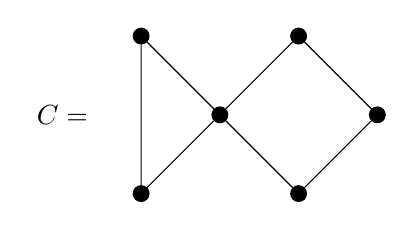
\begin{tikzpicture}[scale=1]
\def\labelsep{0.2}
\node[vertex] (W0) at (0,0){};
\node[vertex] (W1) at (-1,1){};
\node[vertex] (W2) at (-1,-1){};
\node[vertex] (V1) at (1,1){};
\node[vertex] (V2) at (2,0){};
\node[vertex] (V3) at (1,-1){};

\draw (W0) -- (W1) -- (W2) -- (W0) -- (V1) -- (V2) -- (V3) -- (W0);

\node at (-2,0) {$C=$};

\end{tikzpicture}\end{center}Now, let $H$ be a disjoint union of $n_{0}$ copies of the following
graph with maximum degree 4.\begin{center}
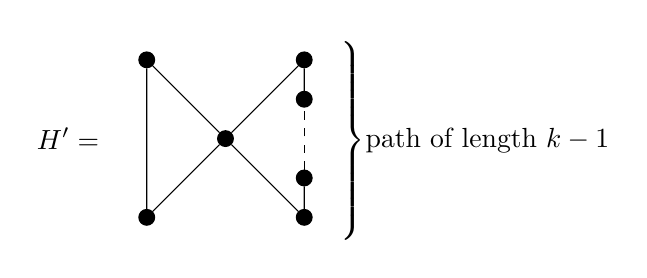
\begin{tikzpicture}[scale=1]
\def\labelsep{0.2}
\node[vertex] (W0) at (0,0){};
\node[vertex] (W1) at (-1,1){};
\node[vertex] (W2) at (-1,-1){};
\node[vertex] (V1) at (1,1){};
\node[vertex] (V2m) at (1,0.5){};
\node[vertex] (V2p) at (1,-0.5){};
\node[vertex] (V3) at (1,-1){};

\draw (V2p) -- (V3) -- (W0) -- (W1) -- (W2) -- (W0) -- (V1) -- (V2m);
\draw [dashed] (V2p) -- (V2m);

\node [align=left,anchor=west] at (1.3,0) {$\left.\rule{0pt}{40pt}\right\}\text{path of length $k-1$}$};

\node at (-2,0) {$H'=$};

\end{tikzpicture}\end{center}The conditions on the $n_{i}$ ensure that $H$ is embeddable in the
complete blow-up $b\left(C\right)$. Specifically, to embed each copy
of $H'$ in $b\left(C\right)$, embed the triangular part using the
clusters $W_{i}$, then embed the $\left(k-1\right)$-path zigzagging
through the clusters $V_{i}$. By the blow-up lemma, for small $\varepsilon$
the super-regular blow-up $b_{\varepsilon,\delta}\left(C\right)$
contains $H$ as well. This embedding of $H$ into $b_{\varepsilon,\delta}\left(C\right)$
must be of the same type as our embedding into $b\left(C\right)$:
the triangular part of $H'$ can only be embedded using the clusters
$W_{i}$, and embedding all $n_{0}$ of these triangular parts uses
up all the vertices in the $W_{i}$. Therefore the embeddings of the
$k$-cycle part of $H'$ give us the special paths in $G$ we require.

\textbf{This seems like a silly way to apply the blow-up lemma...
I add the 3-cycle just to make sure my $\boldsymbol{k}$-cycles are
embedded in the ``right'' way. Is there a better way to guarantee
this?}
\end{proof}
It remains to explain the ``adjustments'' necessary to apply the
above two lemmas. For both, we make use of the following lemma $O\left(1\right)$
times, repeatedly removing sets of ``adjusting'' special paths.
\begin{lem}
\label{lem:adjusting-paths}For any $\delta<0$, $f<1$, and any integer
$k>2$ there is $\delta'=\delta'\left(\delta\right)>0$ and $\c=\c\left(\delta,f,k\right)$
such that the following holds. Let $\G$ be a graph on some vertex
set $\range N$, together with a vertex partition into $O\left(1\right)$
clusters, such that some of the pairs of clusters $\left(V,W\right)$
are $\left(\varepsilon,\delta\right)$-super-regular. Consider any
sequence of clusters $V_{0},\dots,V_{k}$, such that $\left(V_{0},V_{1}\right)$
and $\left(V_{k-1},V_{k}\right)$ are $\left(\varepsilon,\delta\right)$-super-regular
pairs, and such that if a cluster appears in the sequence $t$ times,
then it has at least $tn$ vertices. Suppose further that each $\x\in V_{0}$
is bijectively paired with a vertex $\y\in V_{k}$, comprising a special
pair $\left(\x,\y\right)$. Let $\R\in\GG\left(n,\c/n\right)$. Then
for any $m\le fn$, there are $m$ vertex-disjoint special paths of
the form $v_{1}\dots v_{k}$ ($v_{i}\in V_{i}$) in $\G\cup\R$. Let
$P$ be the union of our special paths; we can choose these paths
in such a way that $\left(V\backslash P,W\backslash P\right)$ is
$\left(\varepsilon,\delta'\right)$-super-regular for each $\left(V,W\right)$
that was $\left(\varepsilon,\delta\right)$-super-regular (in $\G$).
\end{lem}
We also give a simplified form of the same lemma, which we will use
in the proof of \ref{lem:adjusting-paths}.
\begin{lem}
\label{lem:easy-adjusting-paths}For any $\delta>0$, $g<1$ and $k\in\NN$,
there is $\c=\c\left(\delta,p,k\right)$ such that the following holds.
Let $\G$ be a graph on the vertex set $\range{kn}$, together with
a vertex partition $\range{kn}=V_{0}\cup\dots\cup V_{k}$. Suppose
that each $\left|V_{i}\right|=n$, and each $v\in V_{0}$ (respectively,
$v\in V_{k}$) has at least $\delta n$ neighbours in $V_{2}$ (respectively,
in $V_{k-1}$). Suppose further that each $\x\in V_{0}$ is bijectively
paired with a vertex $\y\in V_{k}$, comprising a special pair $\left(\x,\y\right)$.
Let $\R\in\GG\left(n,\c/n\right)$. Then there are a.a.s. $gn$ vertex-disjoint
special paths of the form $v_{1}\dots v_{k}$ ($v_{i}\in V_{i}$)
in $\G\cup\R$.\end{lem}
\begin{proof}
It suffices to show that we can a.a.s. find $\varepsilon n$ such
disjoint paths, for any small $\varepsilon=\varepsilon\left(\delta\right)>0$.
This is because we can break $\R$ into phases $\R\supseteq\R_{1}\cup\dots\cup\R_{r}$,
where $r$ is chosen so that $\left(1-\varepsilon\right)^{r}\le\left(1-g\right)$.
Each phase we can cover an $\varepsilon$-fraction of the vertices
with suitable $k$-paths; discard these paths for the next phase and
repeat.

We proceed with this plan, for $\varepsilon=\delta^{3}/\left(2\sqrt{2}\right)$.
For any $\gamma=\gamma\left(\delta\right)>0$, by \ref{lem:bipartite-matching}
we can find a matching of $\left(1-\left(1-\gamma\right)/\left(k-2\right)\right)n$
edges between each $V_{i}$ and $V_{i+1}$ ($1\le i<k-1$). This gives
us a disjoint union of $\gamma n$ paths $P_{1},\dots,P_{\gamma n}$
in $\G\cup\R$, where $P_{i}=v_{1}^{i}\dots v_{k-1}^{i}$ (with $v_{j}^{i}\in V_{j}$).
We can assume that $v_{j}^{1},\dots,v_{j}^{\gamma n}$ is a uniformly
random ordering of a uniformly random set of $\gamma n$ elements
of $V_{j}$ (independently for $2\le j\le k-1$).

Now, let the special pairs be $\left(\x^{1},\y^{1}\right),\dots,\left(\x^{n},\y^{n}\right)$.
Note that $\Pr\left(v_{1}^{1}\sim\x^{1},v_{k-1}^{1}\sim\y^{1}\right)\ge\delta^{2}$
and more generally, 
\[
\Pr\left(v_{1}^{i}\sim\x^{i},v_{k-1}^{i}\sim\y^{i}\mid v_{1}^{1},v_{k-1}^{1},\dots,v_{1}^{\gamma n},v_{k-1}^{\gamma n}\right)\ge\left(\left(\delta n\right)^{2}-i^{2}\right)/n^{2}\ge\delta^{2}/2
\]
for all $i\le\gamma n$, with $\gamma=\delta n/\sqrt{2}$. By the
Chernoff bound, there are a.a.s. $\delta^{3}n/\left(2\sqrt{2}\right)$
special paths $\x_{i},v_{1}^{i},\dots,v_{k-1}^{i},\y_{i}$.
\end{proof}

\begin{proof}[Proof of \ref{lem:adjusting-paths}]
First note that we can assume each $V_{i}$ is distinct. For, we
can take every cluster that appears multiple times (say $t$ times)
in the sequence and split that cluster into $t$ equal-sized subclusters
uniformly at random. Since $t\le k=O\left(1\right)$, by \ref{lem:random-preserves-superregular}
super-regularity is a.a.s. preserved by these splits. That is, if
$\left(V,W\right)$ was $\left(\varepsilon,\delta\right)$-super-regular
in $\G$, and $V'\subseteq V$, $W'\subseteq W$ are clusters after
the splits, then $\left(V',W'\right)$ is a.a.s. $\left(\varepsilon,\delta/2\right)$-super-regular.

So we proceed with distinct $V_{i}$. For each $V_{i}$, set aside
a uniformly random subset $D_{i}$ of size $\left(\left|V_{i}\right|-m\right)/2$.
Let $U_{i}=V_{i}\backslash D_{i}$ so that $\left|V_{i}\backslash D_{i}\right|\ge n/2$
and $m\le2f\left|V_{i}\backslash D_{i}\right|/\left(1+f\right)$.
Apply \ref{lem:easy-adjusting-paths} with $g=2f/\left(1+f\right)$
to find $m$ special paths in $\G\cup\R$ through the clusters $V_{0}\backslash D_{0},\dots V_{k}\backslash D_{k}$.
Note that each $\left|V_{i}\backslash P\right|=2\left|D_{i}\right|$.
For each $\left(\varepsilon,\delta\right)$-super-regular pair $\left(V_{i},V_{j}\right)$
(respectively $\left(V_{i},W\right)$), by \ref{lem:random-preserves-superregular}
$\left(D_{i},D_{j}\right)$ (respectively $\left(D_{i},W\right)$)
is a.a.s. $\left(\varepsilon,\delta/2\right)$-super-regular, so that
$\left(V_{i}\backslash P,V_{j}\backslash P\right)$ (respectively
$\left(V_{i}\backslash P,W\right)$) is $\left(\varepsilon,\delta/4\right)$-super-regular,
as required.
\end{proof}

\begin{proof}[Proof of \ref{lem:connect-within}]
First consider the case where $n_{0}+n_{2}>n_{1}+n_{3}$. By the
constraints on the $n_{i}$, we have $n_{2}\le\left(k-5\right)n_{0}$
and $n_{0}+n_{2}-\left(n_{1}+n_{3}\right)\le\left(k-6\right)n_{0}$.
With $f=\frac{k-6}{k-4}$, we can find $\floor{\frac{n_{0}+n_{2}-\left(n_{1}+n_{3}\right)}{k-4}}$
disjoint special paths through the clusters 
\[
V_{0},V_{1},\underbrace{V_{2},\dots,,V_{2}}_{k-3},V_{3},V_{4}.
\]
Let $q=\left(k-4\right)\left\langle \frac{n_{0}+n_{2}-\left(n_{1}+n_{3}\right)}{k-4}\right\rangle $
(where $\left\langle \cdot\right\rangle $ gives the fractional part
of a real number). From the vertices that remain after removing the
paths so far, apply \ref{lem:adjusting-paths} again with a small
$\sigma$ to find a single path through the clusters
\[
V_{0},\underbrace{V_{1},\dots,V_{1}}_{\left(k-2-q\right)/2},\underbrace{V_{2},\dots,V_{2}}_{\left(k-2+q\right)/2},V_{3},V_{4}
\]
or through
\[
V_{0},V_{1},\underbrace{V_{2},\dots,V_{2}}_{\left(k-2+q\right)/2},\underbrace{V_{3},\dots,V_{3}}_{\left(k-2-q\right)/2},V_{4}
\]
(one of these is possible). After removing all the adjusting paths
the conditions for \ref{lem:connect-blowup} are satisfied, and \ref{lem:connect-blowup}
ensures that we can finish connecting the special pairs.

The case $n_{0}+n_{2}<n_{1}+n_{3}$ is almost identical. Remove many
paths through the clusters 
\[
V_{0},V_{1},\underbrace{V_{3},\dots,,V_{3}}_{k-2},V_{4},
\]
then through the clusters
\[
V_{0},\underbrace{V_{1},\dots,,V_{1}}_{k-2},V_{3},V_{4},
\]
then clean up by removing a single path before applying \ref{lem:connect-blowup}.
\end{proof}
Now, we conclude the proof of \ref{thm:main-theorem}: recall that
we are trying to remove paths from the clusters $S_{j}^{i}$ using
$\R_{3}$, in order to apply \ref{lem:connect-within} with $\R_{4}$.
This proceeds in the same way as the adjusting path arguments in the
proof of \ref{lem:connect-within}.

Suppose $\left|S_{j}^{1}\cup S_{j}^{2}\cup S_{j}^{3}\right|+m\ge\left(k-1\right)\left|S_{j}^{0}\right|$
and $\left|S_{r}^{1}\cup S_{r}^{2}\cup S_{r}^{3}\right|-m\le\left(k-1\right)\left|S_{j'}^{0}\right|$
for some $j,r$, where one of these inequalities is an equality. Then
use Lemma \ref{lem:adjusting-paths} with $f=1-a'/\left(bk\right)$
to find $\floor{m/\left(k-3\right)}$ paths through the clusters 
\[
S_{r}^{0},S_{r}^{1},\underbrace{S_{j}^{2},\dots,S_{j}^{2}}_{k-3},S_{r}^{3},S_{r}^{4}.
\]
After removing these paths (plus an additional ``cleanup path'')
to obtain clusters $F_{j}^{i}$, we have $\left|F_{g}^{1}\cup F_{g}^{2}\cup F_{g}^{3}\right|=\left(k-1\right)\left|F_{g}^{0}\right|$
for some $g\in\left\{ j,r\right\} $, and still each $\left|F_{g}^{1}\right|,\left|F_{g}^{3}\right|\ge2\left|F_{g}^{0}\right|$.
After removing paths in this way $q=O\left(1\right)$ times, the conditions
for \ref{lem:connect-within} are satisfied for each cluster-path.

\textbf{These ``adjusting path'' arguments are extremely unwiedly.
Maybe there's some different way to express the situation that makes
it easier to state what I'm doing?}

\bibliographystyle{amsplain}
\bibliography{references}

\end{document}
